\documentclass[12pt,a4paper]{article}
\usepackage[utf8]{inputenc}
\usepackage[T1]{fontenc}
\usepackage{graphicx}
\usepackage[table,dvipsnames]{xcolor}
\usepackage[hypertexnames=false,bookmarksnumbered=true]{hyperref}
\usepackage{enumitem}
\usepackage{titlesec}
\usepackage{geometry}
\usepackage{booktabs}
\usepackage{array}
\usepackage{multirow}
\usepackage{tikz}
\usepackage{amssymb}
\usepackage{rotating}
\usepackage{adjustbox}
\usepackage{pdflscape}
\usepackage{longtable}
\usepackage{float}
\usepackage{colortbl}
\usepackage{tcolorbox}
\usepackage{caption}
\usepackage{setspace}
\usepackage{fancyhdr}
\tcbuselibrary{skins}
\usetikzlibrary{shapes,arrows,positioning,fit,backgrounds}
\usepackage{tabularx} % For dynamic table widths

% Page layout optimization
\geometry{a4paper, margin=2.3cm, headheight=15pt, heightrounded}
\setlength{\parindent}{0pt}
\setlength{\parskip}{8pt}

% Improved table formatting
\renewcommand{\arraystretch}{1.2}
\setlength{\tabcolsep}{4pt}

% Better spacing in lists
\setlist{itemsep=3pt, parsep=0pt, listparindent=\parindent, leftmargin=*}

% Better caption formatting
\captionsetup{font=small, labelfont=bf, skip=8pt, width=0.9\textwidth}

% Float placement optimization
\renewcommand{\topfraction}{0.9}
\renewcommand{\bottomfraction}{0.8}
\renewcommand{\textfraction}{0.1}
\renewcommand{\floatpagefraction}{0.7}
\setcounter{topnumber}{3}
\setcounter{bottomnumber}{2}
\setcounter{totalnumber}{5}

% Header and footer setup
\pagestyle{fancy}
\fancyhf{}
\renewcommand{\headrulewidth}{0.4pt}
\renewcommand{\footrulewidth}{0.4pt}
\fancyhead[L]{IFPE - Chatbot com IA}
\fancyhead[R]{Plano de Implantação}
\fancyfoot[C]{\thepage}

% Redefine clear double page to avoid blank pages if needed
\let\cleardoublepage\clearpage

% Section formatting
\titleformat{\section}
  {\normalfont\Large\bfseries\color{blue!80!black}}{\thesection}{1em}{}
\titleformat{\subsection}
  {\normalfont\large\bfseries\color{blue!60!black}}{\thesubsection}{1em}{}
\titleformat{\subsubsection}
  {\normalfont\normalsize\bfseries\color{blue!40!black}}{\thesubsubsection}{1em}{}
  
% Float placement preferences
\renewcommand{\topfraction}{0.85}
\renewcommand{\bottomfraction}{0.85}
\renewcommand{\textfraction}{0.1}
\renewcommand{\floatpagefraction}{0.75}

% Better caption styling
\captionsetup{font=small,labelfont=bf,justification=centering,margin=1cm}

\hypersetup{
    colorlinks=true,
    linkcolor=blue,
    filecolor=magenta,      
    urlcolor=cyan,
    pdftitle={Plano de Implantação - Chatbot com IA para Processos de Segurança do Trabalho IFPE},
    pdfauthor={Maria Beatriz Martins (Bia), Pedro Balbino, Eric Barreto, Lucas Lucena, Sara Pereira, Luis Felipe Guedes},
}

\begin{document}

\begin{titlepage}
    \thispagestyle{empty}
    \centering
    \vspace*{0.5cm}
    % Uncomment the line below when you have the actual logo file
    {\includegraphics[width=4cm]{images/UFPE.jpg}\par}
    \vspace{1cm}
    {\scshape\LARGE Instituto Federal de Pernambuco \par}
    \vspace{1.5cm}
    {\huge\bfseries Plano de Implantação \par}
    \vspace{1cm}
    {\Large\itshape Chatbot com IA para Processos de Segurança do Trabalho\par}
    \vfill
    \begin{center}
    \begin{tabular}{c}
        {\large \textbf{Elaborado por:}}\\[0.5cm]
        Pedro Henrique Souza Balbino\\
        Eric Bezerra Londres Barreto\\
        Lucas Lucena Xavier de Morais\\
        Sara Simone Emilay de Araujo Pereira\\
        Luis Felipe Guedes Souto Moreira\\
        Maria Beatriz Martins Pontes Gonçalo\\
        Pablo Henrique Ferreira da Silva\\
        Vinicius Nobre da Silva Prazeres
    \end{tabular}
    \end{center}
    \vfill
    {\large Abril de 2025\par}
\end{titlepage}

\newpage
\thispagestyle{empty}
\section*{Histórico de Revisões}

\begin{table}[htbp]
\centering
\renewcommand{\arraystretch}{1.3}
\resizebox{\textwidth}{!}{
\begin{tabular}{|c|c|p{8cm}|c|}
\hline
\rowcolor{gray!15}\textbf{Revisão} & \textbf{Data} & \textbf{Descrição} & \textbf{Autor} \\
\hline
1 & 25/03/2025 & Versão inicial do documento & Pedro Balbino \\
\hline
2 & 01/04/2025 & Revisão com incorporação de feedback do cliente & Eric Barreto \\
\hline
3 & 05/04/2025 & Versão final para apresentação & Equipe do Projeto \\
\hline
\end{tabular}
}
\end{table}

\clearpage
\tableofcontents
\thispagestyle{empty}
\clearpage

\section{Introdução}

\subsection{A Organização}
O Instituto Federal de Educação, Ciência e Tecnologia de Pernambuco (IFPE) é uma instituição de ensino superior pública federal vinculada ao Ministério da Educação. Fundado em 2008 a partir da integração do Centro Federal de Educação Tecnológica de Pernambuco (CEFET-PE) e das Escolas Agrotécnicas Federais, o IFPE atualmente possui 16 campi distribuídos por todo o estado de Pernambuco, oferecendo educação profissional, científica e tecnológica de qualidade, em diferentes modalidades e níveis de ensino.

Com aproximadamente 18.000 alunos e 2.500 servidores (docentes e técnicos administrativos), o IFPE tem como missão promover a educação profissional, científica e tecnológica, em todos os seus níveis e modalidades, com base no princípio da indissociabilidade das ações de Ensino, Pesquisa e Extensão, comprometida com uma prática cidadã e inclusiva, de modo a contribuir para a formação integral do ser humano e para o desenvolvimento sustentável da sociedade.

\subsection{O projeto e seu propósito}
O projeto consiste na implementação de um chatbot com Inteligência Artificial destinado a automatizar processos de segurança do trabalho no IFPE. O propósito principal é melhorar a comunicação e a gestão dos processos relacionados à área de segurança do trabalho, fornecendo uma plataforma unificada que centralize informações, automatize o preenchimento de formulários e oriente os usuários durante solicitações relacionadas à segurança do trabalho.

Os objetivos específicos do projeto incluem:

\begin{itemize}
    \item Centralizar a documentação técnica de segurança do trabalho em um repositório de fácil acesso
    \item Automatizar o preenchimento de formulários para reduzir erros e retrabalho
    \item Padronizar os processos de solicitação relacionados à segurança do trabalho
    \item Diminuir a carga de trabalho administrativo da equipe técnica do SIASS
    \item Melhorar a experiência dos servidores ao interagir com o setor de segurança do trabalho
    \item Garantir o cumprimento de normas e procedimentos de segurança
\end{itemize}

\subsection{Equipe do projeto}
A equipe responsável pela elaboração deste plano de implantação e pela condução do projeto é composta por:

\begin{table}[htbp]
\centering
\begin{tabular}{|p{5cm}|p{8cm}|}
\hline
\textbf{Nome} & \textbf{Função no Projeto} \\
\hline
Pedro Henrique Souza Balbino & Analista de Processos / Gerente de Projeto \\
\hline
Eric Bezerra Londres Barreto & Arquiteto de Soluções / Especialista em IA \\
\hline
Lucas Lucena Xavier de Morais & Desenvolvedor / Integração de Sistemas / Gestor desse último ciclo \\
\hline
Sara Simone Emilay de Araujo Pereira & Analista de Requisitos / Gestão da Mudança \\
\hline
Luis Felipe Guedes Souto Moreira & Desenvolvedor / Engenheiro de Dados \\
\hline
Maria Beatriz Martins Pontes Gonçalo & Designer de UX/UI / Gestora desse último ciclo \\
\hline
Pablo Henrique Ferreira da Silva & Especialista em Segurança da Informação \\
\hline
Vinicius Nobre da Silva Prazeres & Analista de Qualidade / Testes \\
\hline
\end{tabular}
\end{table}

\pagebreak

\begin{itemize}
    \item Mauro César de Oliveira (Especialista em Segurança do Trabalho - SIASS/IFPE)
    \item Marco Antônio Eugênio Araujo (Representante SIASS/Cliente)
    \item Equipe do Núcleo de Tecnologia da Informação (NTI) do IFPE
\end{itemize}

\section{Contexto da unidade em estudo}

\subsection{Histórico da unidade de negócio}
O Subsistema Integrado de Atenção à Saúde do Servidor (SIASS) foi instituído pelo Decreto nº 6.833, de 29 de abril de 2009, como parte da Política de Atenção à Saúde e Segurança do Trabalho do Servidor Público Federal (PASS). Sua principal função é coordenar e integrar ações e programas nas áreas de assistência à saúde, perícia oficial, promoção, prevenção e acompanhamento da saúde dos servidores da administração federal.

No IFPE, a unidade SIASS atende não apenas aos servidores da própria instituição, mas também a diversos órgãos públicos federais da região, conforme evidenciado na ata de reunião de 06 de fevereiro de 2025: \textit{"O SIASS atende vários órgãos públicos federais para otimizar recurso financeiro orçamentário. É um órgão dividido compartilhado por vários órgãos e ele está no IFPE, mas atende vários órgãos públicos, dentre eles o próprio IFPE mais polícia rodoviária."} 

O setor de Segurança do Trabalho, foco deste projeto, é um dos componentes do SIASS e tem como responsabilidade garantir condições seguras e saudáveis no ambiente de trabalho, através de avaliações de risco, emissão de laudos técnicos, treinamentos e orientações aos servidores.

\subsection{Principais stakeholders}
Os principais stakeholders envolvidos no escopo do projeto são:

\begin{table}[ht]
\centering
\begin{tcolorbox}[enhanced, colback=white, colframe=gray!40, arc=4mm, boxrule=1pt, width=0.95\textwidth]
\begin{tabular}{|p{3.5cm}|p{9.5cm}|}
\hline
\textbf{Stakeholder} & \textbf{Papel no Projeto} \\
\hline
\textbf{Equipe técnica de Segurança do Trabalho do SIASS} & Responsável pela avaliação de ambientes laboratoriais, emissão de laudos técnicos, gestão de EPIs e análise de riscos ocupacionais. São os usuários primários da plataforma em seu papel administrativo. \\
\hline
\textbf{Servidores do IFPE} & Docentes, técnicos administrativos e outros colaboradores que necessitam interagir com o setor de segurança do trabalho para solicitar avaliações, relatórios, documentos ou orientações. \\
\hline
\textbf{Funcionários terceirizados} & Prestadores de serviço que atuam nas instalações do IFPE e que também estão sujeitos às normas de segurança do trabalho. \\
\hline
\textbf{Gestores departamentais} & Responsáveis pela aprovação e acompanhamento de solicitações relacionadas à segurança do trabalho em suas respectivas áreas. \\
\hline
\textbf{Núcleo de Tecnologia da Informação (NTI)} & Área responsável pela infraestrutura tecnológica do IFPE e pelo suporte técnico à solução a ser implementada. \\
\hline
\textbf{Alta administração do IFPE} & Reitoria e pró-reitorias que definem diretrizes e políticas institucionais, além de aprovar recursos para projetos estratégicos. \\
\hline
\end{tabular}
\end{tcolorbox}
\caption{Mapeamento de Stakeholders do Projeto}
\end{table}

\subsection{Objetivos da unidade de negócio}
Os objetivos do setor de Segurança do Trabalho do SIASS/IFPE incluem:

\begin{itemize}
    \item Garantir a saúde e segurança dos servidores no ambiente de trabalho
    \item Prevenir acidentes e doenças ocupacionais através de medidas preventivas
    \item Assegurar o cumprimento das normas regulamentadoras e legislação de segurança do trabalho
    \item Realizar avaliações de ambientes e emitir laudos técnicos
    \item Desenvolver e implementar programas de prevenção de riscos ambientais
    \item Proporcionar treinamentos e orientações sobre segurança do trabalho
    \item Investigar e analisar acidentes de trabalho
    \item Gerenciar a concessão de adicionais ocupacionais
    \item Fornecer documentação necessária para processos de aposentadoria especial
\end{itemize}

O setor enfrenta desafios significativos devido à equipe reduzida e à alta demanda de serviços, conforme destacado na reunião de 06 de fevereiro de 2025: \textit{"A equipe de César é pequena e ele tem muita demanda então acaba que esse tratamento Inicial [...] é um problema."}

\subsection{Valores de Negócio}

A seguir, apresentamos os valores de negócio identificados para o projeto, conforme a "Prática 4 - SGE e Valores de Negócio":

\begin{table}[htbp]
\centering
\resizebox{\textwidth}{!}{
\begin{tabular}{|p{2cm}|p{4cm}|p{4cm}|p{4cm}|}
\hline
\rowcolor{gray!15}\textbf{Dimensão} & \textbf{Problema} & \textbf{Solução Proposta} & \textbf{Valor de Negócio} \\
\hline
P, Pr, Tec & Dificuldade dos servidores e terceirizados em acessar informações de segurança & Chatbot acessível para todos & Relacionamento mais estreito com clientes, novos modelos de negócio, eficiência operacional \\
\hline
P, Pr & Falta de canal anônimo para denúncias & Implementação de recurso para denúncias anônimas & Melhor tomada de decisões, novos modelos de negócio \\
\hline
Pr & Fluxo burocrático lento para registro de acidentes & Automação dos formulários e direcionamento ágil & Excelência operacional \\
\hline
Pr, Tec & Dificuldade na atualização e centralização de documentos de segurança & Plataforma unificada para rápido acesso & Excelência operacional, novos modelos de negócio \\
\hline
Pr, Tec & Ausência de fluxo automatizado para solicitações de inspeções & Formulários inteligentes integrados ao chatbot & Excelência operacional \\
\hline
Pr & Necessidade de conformidade com normas legais de segurança & Automação da análise e alertas para conformidade & Sobrevivência \\
\hline
Tec, P & Dificuldade no acompanhamento do status das solicitações & Painel de monitoramento com notificações automáticas & Melhor tomada de decisões, relacionamento mais estreito com clientes \\
\hline
\end{tabular}
}
\caption{Valores de Negócio Identificados para o Projeto}
\end{table}

\subsection{Sistema/solução atualmente implantado(a)}
Atualmente, o setor de Segurança do Trabalho do SIASS utiliza uma combinação de sistemas e processos manuais para gerenciar suas atividades:

\begin{itemize}
    \item \textbf{Sistema Eletrônico de Informação (SEI):} Utilizado para a tramitação de processos e documentos oficiais. Conforme mencionado na ata de reunião de 11 de março de 2025, o SEI é o \textit{"principal sistema utilizado atualmente para trâmite de processos e documentos oficiais no IFPE."} No entanto, o sistema não foi concebido especificamente para a gestão de segurança do trabalho e apresenta limitações para este fim.
    
    \item \textbf{SEAPNET:} Sistema do Governo Federal para registro de acidentes de trabalho, com dados desde 2009, conforme mencionado na ata de reunião de 25 de março de 2025.
    
    \item \textbf{Planilhas e documentos locais:} Grande parte das informações é gerenciada através de documentos Microsoft Word e planilhas Excel armazenadas localmente, sem um sistema centralizado.
    
    \item \textbf{E-mail e telefone:} A comunicação com os solicitantes e entre departamentos é frequentemente realizada por e-mail ou telefone, sem padronização ou registro sistemático.
    
    \item \textbf{Formulários físicos:} Diversos processos ainda utilizam formulários em papel que precisam ser preenchidos manualmente.
    
    \item \textbf{Site institucional:} Uma seção do site do IFPE é utilizada para disponibilizar alguns documentos relacionados à segurança do trabalho, mas com limitações quanto à atualização e facilidade de acesso.
\end{itemize}

O especialista em segurança do trabalho, Sr. César, relatou que o sistema SEI é inadequado para a gestão de documentos de segurança, pois \textit{"é voltado para processos que têm início e fim, enquanto documentos de segurança são contínuos e precisam ser constantemente atualizados"} (Ata de reunião de 25 de março de 2025).

\newpage
\section{Análise de estados}

\subsection{Estado Atual}

\subsubsection{Escopo do processo}
O escopo atual dos processos de segurança do trabalho no IFPE engloba uma série de atividades essenciais para garantir a saúde e segurança dos servidores. Com base no documento "Mapeamento de Processos de Segurança aplicáveis ao IFPE" e nas atas de reunião, foram identificados os seguintes macroprocessos:

\begin{itemize}
    \item Gestão de Acidentes do Trabalho
    \item Gestão de Mapeamento e Graduação de Riscos
    \item Gestão de Equipamentos de Proteção Individual (EPIs)
    \item Gestão de Treinamento de SST
    \item Gestão do Plano de Emergência
    \item Gestão de Energias Perigosas
    \item Gestão de Auditorias e Inspeções de Segurança
    \item Gestão de Critérios Mínimos para Contratação de Empresas Terceirizadas
    \item Gestão de Mudanças
    \item Gestão de Documentos de SST
    \item Gestão de Uso de Produtos Químicos
    \item Gestão de Projetos de Novas Instalações com foco em SST
    \item Gestão de concessão de adicionais ocupacionais
    \item Gestão de documentos de aposentadoria especial (PPP)
\end{itemize}

Cada um desses macroprocessos é composto por diversos subprocessos e atividades, que atualmente são executados de forma fragmentada e com baixo grau de automação.

O processo atual consiste no atendimento manual às solicitações de segurança do trabalho, iniciando quando um servidor público envia uma demanda ao servidor do SIASS por meio de e-mail ou via SEI. O servidor do SIASS verifica manualmente as informações recebidas e, caso identifique dados incompletos, solicita o reenvio das informações faltantes ao servidor solicitante, prolongando o tempo de resposta.

Uma vez validada a solicitação, o servidor do SIASS abre o processo manualmente e entra em contato com o servidor público para coletar detalhes adicionais, utilizando canais não padronizados (e-mail, ligação telefônica ou mensagens via aplicativos). Após essa etapa, o servidor do SIASS agenda a visita técnica, comunica o solicitante e aguarda confirmação.

Na data agendada, a visita técnica é realizada, e, posteriormente, o servidor do SIASS elabora manualmente o relatório, o registra no SEI e notifica o servidor público sobre a conclusão do processo. Por fim, o documento é arquivado, encerrando o fluxo.

\subsubsection{Processos - As Is (Modelagem dos processos atualmente implementados)}

Este fluxo de trabalho atual pode ser descrito em quatro etapas principais:

\begin{enumerate}
    \item \textbf{Iniciação do Processo:}
    \begin{itemize}
        \item Abertura de processo no sistema SEI
        \item Documentação inicial frequentemente incompleta
        \item Ausência de padronização nas solicitações
    \end{itemize}
    
    \item \textbf{Coleta de Informações:}
    \begin{itemize}
        \item Processo manual de entrevistas
        \item Uso de canais informais (telefone pessoal, e-mail)
        \item Documentação em papel durante visitas
    \end{itemize}
    
    \item \textbf{Análise Técnica:}
    \begin{itemize}
        \item Visita presencial ao local
        \item Avaliação baseada em normas técnicas
        \item Consulta a especialistas quando necessário
    \end{itemize}
    
    \item \textbf{Documentação:}
    \begin{itemize}
        \item Elaboração de relatório em Word
        \item Inclusão no sistema SEI
        \item Arquivamento do processo
    \end{itemize}
\end{enumerate}

\begin{landscape}
\begin{figure}[p]
\centering
\includegraphics[width=0.85\paperwidth, height=0.8\paperheight, keepaspectratio]{images/AS-IS.jpg}
\caption{Processo Atual (As-Is) de Solicitação de Segurança do Trabalho. \\ Diagrama original: \url{https://lucid.app/lucidchart/40645f0c-1a65-4212-8d42-41b5854b891d/edit?invitationId=inv_0024c9b9-9c9b-470f-a54f-679cf3aab54d&page=QSIJBMCcx_hD}}
\end{figure}
\end{landscape}


Este processo As-Is apresenta diversas ineficiências e pontos de gargalo, conforme identificado nas reuniões com o cliente:

\begin{enumerate}
    \item \textbf{Iniciação do Processo:}
    \begin{itemize}
        \item Abertura de processo no sistema SEI
        \item Documentação inicial frequentemente incompleta
        \item Ausência de padronização nas solicitações
    \end{itemize}
    
    \item \textbf{Coleta de Informações:}
    \begin{itemize}
        \item Processo manual de entrevistas
        \item Uso de canais informais (telefone pessoal, e-mail)
        \item Documentação em papel durante visitas
    \end{itemize}
    
    \item \textbf{Análise Técnica:}
    \begin{itemize}
        \item Visita presencial ao local
        \item Avaliação baseada em normas técnicas
        \item Consulta a especialistas quando necessário
    \end{itemize}
    
    \item \textbf{Documentação:}
    \begin{itemize}
        \item Elaboração de relatório em Word
        \item Inclusão no sistema SEI
        \item Arquivamento do processo
    \end{itemize}
\end{enumerate}

\subsubsection{Vantagens: O que é bom?}
Apesar das ineficiências identificadas, o processo atual apresenta algumas vantagens que devem ser preservadas na nova solução:

\begin{itemize}
    \item \textbf{Experiência e conhecimento técnico da equipe:} A equipe de segurança do trabalho possui profundo conhecimento técnico e experiência acumulada ao longo dos anos, o que garante a qualidade das análises e pareceres emitidos.
    
    \item \textbf{Flexibilidade para casos excepcionais:} O processo atual, por ser menos estruturado, permite maior flexibilidade para lidar com situações atípicas ou emergenciais que não se enquadram em fluxos padronizados.
    
    \item \textbf{Contato direto com os solicitantes:} A interação pessoal entre a equipe técnica e os solicitantes possibilita um entendimento mais profundo das necessidades e contextos específicos de cada caso.
    
    \item \textbf{SEI como sistema oficial de registro:} A utilização do SEI como sistema oficial garante a legalidade e rastreabilidade dos processos, além de ser um sistema já conhecido pelos servidores.
    
    \item \textbf{Visitas técnicas presenciais:} As visitas presenciais aos locais de análise permitem uma avaliação mais precisa e contextualizada dos ambientes e riscos.
\end{itemize}

\subsubsection{Desafios: O que pode melhorar?}
A análise do processo atual revelou diversos desafios e oportunidades de melhoria nos processos de segurança do trabalho do IFPE. A seguir, destacamos os principais pontos identificados:

\textbf{Problemas de Comunicação:}

\begin{itemize}
    \item \textbf{Canais Informais:} Atualmente, as entrevistas são realizadas de maneira informal, com anotações feitas manualmente e posteriormente transformadas em documentos de texto.

    \item \textbf{Falta de Padronização:} Os pedidos muitas vezes chegam de forma desestruturada, exigindo contato direto com os solicitantes para entender a demanda, o que gera inconsistência nos processos.

    \item \textbf{Retrabalho Constante:} Informações importantes muitas vezes são registradas tardiamente, o que gera retrabalho para a equipe na consolidação dos dados.

    \item \textbf{Dificuldade de acesso à documentação:} A documentação está dispersa em diferentes sistemas e formatos, dificultando sua localização e utilização.

    \item \textbf{Subnotificação de acidentes:} Pequenos acidentes frequentemente não são registrados por parte dos servidores, seja por receio ou por falta de conhecimento sobre o procedimento adequado.
\end{itemize}

\textbf{Problemas Organizacionais:}

\begin{itemize}
    \item \textbf{Equipe Reduzida:} A equipe responsável é pequena e sobrecarregada, o que compromete o tratamento inicial das demandas.

    \item \textbf{Falta de Recursos Dedicados:} Não há um canal formal e estruturado para o atendimento, o que prejudica a formalização adequada das solicitações.

    \item \textbf{Complexidade das Demandas:} Algumas demandas são altamente técnicas e exigem a consulta a especialistas externos, o que dificulta sua resolução.

    \item \textbf{Sistema SEI inadequado:} O sistema utilizado não é ideal para documentos que exigem atualizações contínuas, como é o caso da documentação de segurança.

    \item \textbf{Falta de digitalização e padronização visual:} A documentação é predominantemente textual, sem o uso de elementos visuais que poderiam facilitar sua compreensão.
\end{itemize}

\subsubsection{Justificativa}

A partir da análise realizada, identificou-se que o problema central no processo atual é a ineficiência no fluxo de solicitações e no acesso à documentação, o que compromete a agilidade e a conformidade dos processos relacionados à segurança do trabalho no SIASS. A causa raiz desse problema é a ausência de um sistema próprio e centralizado para a formalização das solicitações, o que obriga o uso de múltiplos meios de comunicação e favorece o surgimento de processos informais, sem padronização adequada. Entre as causas comuns, destaca-se a falta de padronização das solicitações, que gera retrabalho e consultas manuais para suprir informações ausentes. Além disso, a documentação técnica de difícil acesso nos sistemas atuais dificulta a verificação de detalhes importantes por parte dos profissionais de segurança do trabalho. Como causa especial, observa-se a ausência de integração entre os sistemas e a não disponibilização facilitada de materiais normativos essenciais, o que aumenta a dificuldade para manter a conformidade com as rigorosas normas regulamentadoras da CLT.

\clearpage
\subsection{Estado Desejado}

O estado desejado para os processos de segurança do trabalho no IFPE é caracterizado por um fluxo de trabalho otimizado, digital e centrado no usuário, conforme ilustrado no diagrama TO-BE apresentado anteriormente. Esta nova abordagem resolve os problemas identificados no processo atual e incorpora as seguintes características principais:

\begin{itemize}
    \item \textbf{Interface conversacional intuitiva:} Um chatbot com IA que guia os usuários por todo o processo, desde a solicitação inicial até o acompanhamento do status.
    
    \item \textbf{Preenchimento assistido de formulários:} Sistema inteligente que auxilia no preenchimento correto e completo dos formulários, reduzindo erros e omissões.
    
    \item \textbf{Base de conhecimento centralizada:} Repositório unificado de normas, procedimentos e documentos técnicos, facilmente acessível e pesquisável.
    
    \item \textbf{Integração com o SEI:} Conexão direta com o sistema oficial, mantendo a conformidade legal e eliminando a duplicação de dados.
    
    \item \textbf{Automação de processos:} Fluxos de trabalho automatizados para tarefas repetitivas, liberando a equipe técnica para atividades de maior valor.
    
    \item \textbf{Análise preditiva:} Capacidade de identificar padrões e tendências, permitindo uma abordagem mais proativa à segurança do trabalho.
\end{itemize}

Este estado futuro não apenas elimina as ineficiências do processo atual, mas também oferece novas capacidades que elevam a qualidade e o alcance dos serviços de segurança do trabalho no IFPE.

\subsection{Análise de Gaps}

\begin{table}[htbp]
\caption*{\textbf{Arquitetura de Negócios}}
\centering
\resizebox{0.9\textwidth}{!}{
\begin{tabular}{|p{4cm}|p{4cm}|p{4cm}|p{4cm}|}
\hline
\rowcolor{blue!10}\textbf{Elemento} & \textbf{Estado Atual} & \textbf{Estado Desejado} & \textbf{Gap Identificado} \\
\hline
\textbf{Processos de Negócio} & Processos manuais, fragmentados e com documentação limitada. Múltiplos canais de comunicação não integrados. & Processos automatizados, integrados e com documentação digital completa. Canal unificado de comunicação. & Ausência de automação e padronização nos processos principais de segurança do trabalho. \\
\hline
\textbf{Organização} & Estrutura hierárquica tradicional com comunicação vertical. Equipe técnica reduzida com alta demanda de trabalho. & Estrutura mais horizontal com comunicação direta através do sistema. Equipe técnica focada em atividades de alto valor. & Necessidade de reorganização da distribuição de tarefas e responsabilidades para otimizar recursos humanos limitados. \\
\hline
\textbf{Serviços de Negócio} & Serviços prestados de forma reativa e com documentação manual. Tempo de resposta longo e variável. & Serviços prestados de forma proativa, com documentação automatizada e tempo de resposta previsível. & Falta de capacidade para oferecer serviços proativos e preventivos devido às limitações de recursos e sistemas. \\
\hline
\end{tabular}
}
\caption{Gap Analysis - Principais Domínios de Arquitetura de Negócios}
\end{table}

\begin{table}[htbp]
\centering
\begin{tcolorbox}[enhanced, colback=white, colframe=gray!40, arc=3mm, boxrule=0.5pt, width=0.9\linewidth]
\scriptsize
\resizebox{0.85\textwidth}{!}{
\begin{tabular}{|p{2.2cm}|p{2.4cm}|p{2cm}|p{2.3cm}|p{1.4cm}|p{1.4cm}|p{2cm}|p{1.8cm}|}
\hline
\rowcolor{gray!20}
\textbf{Detalhamento da Mudança} & \textbf{What?} & \textbf{Why?} & \textbf{Who?} & \textbf{Where?} & \textbf{When?} & \textbf{How?} & \textbf{How Much?} \\
\hline
1. Identificação do ESTADO ATUAL dos procedimentos de trabalho & Processo atual de Segurança do Trabalho no SIASS envolve abertura manual de processos, coleta de informações informalmente, documentação final manual. & A equipe é reduzida, a documentação é descentralizada, aumentando o tempo de resposta. & Equipe de Segurança do Trabalho do SIASS, servidores envolvidos no processo. & Ambiente de trabalho do SIASS, incluindo laboratórios e setores administrativos. & Durante a abertura de processos e a realização de inspeções. & Abertura de processos no SEI, entrevistas com especialistas, visita técnica e elaboração de documentos manuais. & Alto — devido ao tempo gasto em coletas de informações e retrabalho. \\
\hline
2. Identificação do NOVO ESTADO, considerando os procedimentos de trabalho já melhorados & Automação inteligente do processo de Segurança do Trabalho, com preenchimento guiado e integração com normas técnicas. & Redução do retrabalho, maior padronização das informações e melhoria na eficiência do processo. & Equipe de Segurança do Trabalho, desenvolvedores do sistema e usuários finais. & Sistema digital implementado no SIASS para gestão de segurança. & Durante a implementação do novo sistema digital. & Uso de tecnologia de preenchimento assistido e integração com normas técnicas. & Médio — custos iniciais de implementação, mas economia no longo prazo. \\
\hline
3. Identificação das LACUNAS ou problemas/falhas do estado atual & Falta de padronização na coleta de informações, retrabalho na documentação e dependência de entrevistas presenciais. & As informações são coletadas de maneira informal, dificultando o processo e gerando inconsistências. & Profissionais do SIASS, equipe administrativa, técnicos de segurança do trabalho. & Atividades presenciais, como entrevistas e inspeções, e atividades administrativas. & No momento de coleta de informações e geração de documentos. & Documentação manual, falta de sistema de preenchimento assistido e alto tempo de resposta. & Alto — elevado custo em tempo de trabalho e inconsistências nos dados. \\
\hline
4. Propostas de MELHORIAS para fechar as lacunas do item 3 & Processo automático para preenchimento de formulários, integração com banco de normas técnicas e automação de laudos técnicos. & Facilitar o preenchimento de formulários, garantir precisão nas informações e reduzir o tempo de análise. & Gestores do SIASS, equipe técnica de TI e profissionais da Segurança do Trabalho. & Ambiente digital, com automatização do fluxo de trabalho e documentação técnica. & Após a implementação do novo sistema automatizado. & Processo automatizado para preenchimento e análise de segurança. & Baixo — otimização do tempo e aumento da produtividade reduzindo erros. \\
\hline
\end{tabular}
}
\end{tcolorbox}
\caption{Análise de Gaps com foco em Processos de Negócio}
\end{table}

\begin{table}[htbp]
\caption*{\textbf{Arquitetura de Sistemas de Informação}}
\centering
\resizebox{0.9\textwidth}{!}{
\begin{tabular}{|p{4cm}|p{4cm}|p{4cm}|p{4cm}|}
\hline
\rowcolor{blue!10}\textbf{Elemento} & \textbf{Estado Atual} & \textbf{Estado Desejado} & \textbf{Gap Identificado} \\
\hline
\textbf{Aplicações} & Sistema SEI para processos gerais. Sem sistema específico para gestão de segurança do trabalho. & Sistema integrado de gestão de segurança com interface conversacional e automação de formulários. & Ausência de aplicação específica para processos de segurança do trabalho e interface mais acessível aos usuários. \\
\hline
\textbf{Integração} & Sistemas isolados sem comunicação automatizada. Transferência manual de informações. & Sistemas integrados com fluxo automatizado de informações e validação de dados. & Falta de interfaces de integração entre sistemas e padrões de interoperabilidade. \\
\hline
\textbf{Usabilidade} & Interfaces complexas, focadas em especialistas. Uso de formulários em papel e digitais não padronizados. & Interface conversacional intuitiva, acessível a todos os níveis de usuários e adaptativa ao contexto. & Alta curva de aprendizado dos sistemas atuais e falta de assistência contextual ao usuário. \\
\hline
\end{tabular}
}
\caption{Gap Analysis - Principais Aspectos dos Sistemas de Informação}
\end{table}

\begin{table}[htbp]
\centering
\begin{tcolorbox}[enhanced, colback=white, colframe=gray!40, arc=3mm, boxrule=0.5pt, width=0.85\linewidth]
\begin{tabular}{|p{2cm}|p{9.5cm}|}
\hline
\rowcolor{gray!20}
\textbf{Etapa} & \textbf{Descrição} \\
\hline
1. Identificação de funcionalidades atuais & Sistema atual: a coleta de informações é feita de forma descentralizada, com uso de artefatos manuais e processos não padronizados. \\
\hline
2. Funcionalidades do novo sistema & O novo sistema proposto visa automatizar o preenchimento assistido de formulários, evoluir para uma plataforma autônoma que interaja com o usuário, integrar normas técnicas e oferecer suporte à decisão na análise de viabilidade, além de centralizar todas as etapas dentro de um ambiente digital estruturado. \\
\hline
3. Lacunas do sistema atual & \begin{itemize}\setlength{\itemsep}{0pt}
\item Falta de padronização e formalização inicial do processo
\item Comunicação informal que gera retrabalho e perda de informações
\item Equipe reduzida sem ferramentas adequadas para otimizar a gestão
\item Documentação fragmentada e descentralizada
\end{itemize} \\
\hline
4. Melhorias propostas & \begin{itemize}\setlength{\itemsep}{0pt}
\item Implementação de um sistema integrado para formalizar a comunicação e as solicitações
\item Digitalização dos processos e automação no preenchimento de formulários
\item Criação de um módulo de suporte à decisão baseado em normas técnicas
\end{itemize} \\
\hline
\end{tabular}
\end{tcolorbox}
\caption{Análise de Gaps com foco em Sistemas de Informação}
\end{table}

\clearpage
\begin{table}[htbp]
\caption*{\textbf{Arquitetura de Dados}}
\centering
\resizebox{\textwidth}{!}{
\begin{tabular}{|p{4cm}|p{4cm}|p{4cm}|p{4cm}|}
\hline
\rowcolor{blue!10}\textbf{Elemento} & \textbf{Estado Atual} & \textbf{Estado Desejado} & \textbf{Gap Identificado} \\
\hline
\textbf{Modelos de Dados} & Dados não estruturados em documentos de texto. Sem modelo centralizado. & Dados estruturados em banco de dados relacional e não-relacional. Base de conhecimento vetorial. & Ausência de estruturação adequada de dados e modelo semântico para gestão do conhecimento. \\
\hline
\textbf{Qualidade de Dados} & Inconsistência entre documentos, informações duplicadas e desatualizadas. & Dados consistentes, validados e com atualização automática. Trilha de auditoria de alterações. & Falta de mecanismos de validação, controle de qualidade e garantia de consistência. \\
\hline
\textbf{Acesso a Dados} & Acesso limitado a documentos físicos ou por e-mail. Difícil recuperação de informações históricas. & Acesso unificado via interface intuitiva. Busca semântica e filtros contextuais. & Ausência de mecanismos de indexação, busca avançada e disponibilização contextual de informações. \\
\hline
\end{tabular}
}
\caption{Gap Analysis - Principais Aspectos da Arquitetura de Dados}
\end{table}

\begin{table}[htbp]
\centering
\begin{tcolorbox}[enhanced, colback=white, colframe=gray!40, arc=3mm, boxrule=0.5pt, width=0.85\linewidth]
\begin{tabular}{|p{2cm}|p{10cm}|}
\hline
\rowcolor{gray!20}
\textbf{Etapa} & \textbf{Descrição} \\
\hline
1. Fontes de dados atuais & \begin{itemize}\setlength{\itemsep}{0pt}
\item \textbf{Documentações técnicas de normas de segurança do trabalho:} Fonte de dados com alta qualidade e facilidade de acesso, disponível em formato digital e físico, sendo pública e regulamentada.
\item \textbf{Documentação em papel das visitas técnicas:} Fonte de dados armazenada de forma manual, com disponibilidade limitada e qualidade potencialmente comprometida devido à dificuldade de atualização.
\item \textbf{Dados de abertura de solicitação de processo:} Fonte de dados mista que pode ser encontrada no sistema SEI ou via email, impactando negativamente na qualidade e confiabilidade dos dados.
\end{itemize} \\
\hline
2. Fontes de dados no novo cenário & \begin{itemize}\setlength{\itemsep}{0pt}
\item \textbf{Documentações técnicas de normas de segurança do trabalho:} Mantém-se como fonte de alta qualidade e facilidade de acesso.
\item \textbf{Documentação das visitas técnicas:} Será armazenada em sistema integrado com o SEI, permitindo maior agilidade no processo, capacidade de alteração das informações e maior disponibilidade de acesso.
\item \textbf{Dados de abertura de solicitação de processo:} Será centralizada e estruturada no sistema integrado.
\end{itemize} \\
\hline
3. Lacunas identificadas & Ausência de integração da documentação manual com o sistema SEI pelo qual será gerado o relatório do processo, além da utilização de recursos manuais na fonte de dados atual, trazendo problemas de disponibilidade por limitação de acesso em meios físicos e qualidade dos dados, além de inibir uma capacidade mais ágil de alteração dos dados. \\
\hline
4. Melhorias propostas & Substituição do método manual da fonte de dados da documentação das visitas técnicas por meios virtuais e integrados com o sistema atual utilizado para a geração de relatório, o sistema SEI. \\
\hline
\end{tabular}
\end{tcolorbox}
\caption{Análise de Gaps com foco em Dados}
\end{table}
\clearpage
\begin{table}[htbp]
\caption*{\textbf{Arquitetura de Tecnologia}}
\centering
\resizebox{\textwidth}{!}{
\begin{tabular}{|p{4cm}|p{4cm}|p{4cm}|p{4cm}|}
\hline
\rowcolor{blue!10}\textbf{Elemento} & \textbf{Estado Atual} & \textbf{Estado Desejado} & \textbf{Gap Identificado} \\
\hline
\textbf{Infraestrutura} & Infraestrutura local com sistemas em servidores institucionais. Acesso principalmente em estações de trabalho. & Infraestrutura híbrida (cloud + on-premises) com alta disponibilidade. Acesso multiplataforma (web, mobile). & Falta de infraestrutura flexível, escalável e acessível através de múltiplos dispositivos. \\
\hline
\textbf{Segurança} & Controle de acesso básico. Sem criptografia avançada ou protocolos robustos de segurança. & Segurança multicamadas com autenticação forte, criptografia, auditoria e conformidade com LGPD. & Deficiências nos mecanismos de proteção de dados sensíveis e controles de segurança avançados. \\
\hline
\textbf{Plataformas Tecnológicas} & Tecnologia tradicional sem recursos de IA ou automação avançada. Pouco uso de APIs. & Plataforma moderna com IA, processamento de linguagem natural, APIs RESTful e microserviços. & Ausência de tecnologias emergentes para automação inteligente e experiência conversacional. \\
\hline
\end{tabular}
}
\caption{Gap Analysis - Principais Aspectos da Arquitetura de Tecnologia}
\end{table}

\begin{table}[htbp]
\centering
\begin{tcolorbox}[enhanced, colback=white, colframe=gray!40, arc=3mm, boxrule=0.5pt, width=0.85\linewidth]
\begin{tabular}{|p{2cm}|p{10cm}|}
\hline
\rowcolor{gray!20}
\textbf{Etapa} & \textbf{Descrição} \\
\hline
1. Arquitetura tecnológica atual & Atualmente, o sistema utilizado é o SEI (Sistema Eletrônico de Informações), que gerencia processos administrativos de forma manual. Além disso, a coleta de informações ocorre via e-mail e telefone, com os relatórios sendo gerados em arquivos Word e armazenados no sistema. \\
\hline
2. Arquitetura tecnológica nova & O novo sistema contará com um módulo de automação inteligente para preenchimento de formulários e análise de segurança do trabalho. Haverá integração com o SEI para armazenamento centralizado, além de um banco de normas técnicas para padronização dos laudos. \\
\hline
3. Lacunas tecnológicas & O sistema atual não possui automação, exigindo intervenção manual em todas as etapas do processo. A coleta de dados é descentralizada e há risco de perda de informações devido ao uso de canais informais. Além disso, não há integração com normas técnicas, o que dificulta a padronização. \\
\hline
4. Melhorias tecnológicas & \begin{itemize}\setlength{\itemsep}{0pt}
\item Implementação de um assistente virtual inteligente para auxiliar no preenchimento de formulários
\item Integração com um banco de normas técnicas para automação de verificações de conformidade
\item Desenvolvimento de um módulo de análise preditiva para reduzir retrabalho e otimizar a tomada de decisão
\end{itemize} \\
\hline
\end{tabular}
\end{tcolorbox}
\caption{Análise de Gaps com foco em Tecnologia}
\end{table}

\begin{table}[htbp]
\caption*{\textbf{Processos e Visualização de Sistemas}}
\centering
\begin{minipage}{0.8\textwidth}
\centering
\fbox{\begin{tabular}{c}
\textbf{Sistema Atual} \\
\\
\begin{tabular}{c|c}
Usuário & Sistema SEI \\
$\downarrow$ & $\downarrow$ \\
Insere dados manualmente & Armazena documentos \\
$\downarrow$ & \\
Recebe resultado & \\
\end{tabular}
\end{tabular}}
\caption{Representação do sistema atual}
\end{minipage}
\end{table}

\begin{table}[htbp]
\centering
\begin{minipage}{0.8\textwidth}
\centering
\fbox{\begin{tabular}{c}
\textbf{Novo Sistema} \\
\\
\begin{tabular}{c}
Usuário \\
$\downarrow$ \\
Interação e fornecimento de dados \\
$\downarrow$ \\
Assistente \\
$\downarrow$ \\
Verificação com Normas Técnicas \\
$\downarrow$ \\
SEI (Sistema Eletrônico de Informações) \\
$\downarrow$ \\
Armazena informações estruturadas \\
$\downarrow$ \\
Interface Web
\end{tabular}
\end{tabular}}
\caption{Representação do novo sistema}
\end{minipage}
\end{table}

\begin{table}[htbp]
\centering
\begin{minipage}{0.8\textwidth}
\centering
\fbox{\begin{tabular}{c}
\textbf{Arquitetura Tecnológica Atual} \\
\\
\begin{tabular}{c}
Usuário \\
$\downarrow$ \\
Email/Telefone $\rightarrow$ SEI \\
$\downarrow$ \\
Documentos Word \\
$\downarrow$ \\
Geração manual de relatórios
\end{tabular}
\end{tabular}}
\caption{Arquitetura tecnológica atual}
\end{minipage}
\end{table}

\begin{table}[htbp]
\centering
\begin{minipage}{0.8\textwidth}
\centering
\fbox{\begin{tabular}{c}
\textbf{Arquitetura Tecnológica Nova} \\
\\
\begin{tabular}{c}
Interface Web/Chatbot \\
$\downarrow$ \\
Módulo de Preenchimento Inteligente \\
$\downarrow$ \\
Banco de Normas Técnicas \\
$\downarrow$ \\
Geração automática de relatórios \\
$\downarrow$ \\
Banco de Dados Centralizado \\
\end{tabular}
\end{tabular}}
\caption{Arquitetura tecnológica nova}
\end{minipage}
\end{table}

\begin{center}
\textbf{Processos - To Be (Modelagem dos processos melhorados)}
\end{center}

O estado desejado prevê uma transformação significativa nos processos de segurança do trabalho, com a implementação do chatbot com IA como ponto central de interação. A seguir, apresentamos a modelagem do processo genérico no estado desejado:

\section{Conclusões e Considerações Finais}

A implantação do chatbot com IA para processos de segurança do trabalho representa uma oportunidade significativa para transformar e modernizar os serviços prestados pelo setor de Segurança do Trabalho do SIASS/IFPE. Este plano de implantação foi elaborado com base em uma análise detalhada do contexto atual, identificação de desafios e oportunidades, e definição de uma estratégia gradual e iterativa para maximizar as chances de sucesso.

Os principais benefícios esperados com a implementação desta solução incluem:

\begin{itemize}
    \item \textbf{Eficiência operacional:} Redução significativa no tempo de processamento de solicitações e no esforço administrativo da equipe técnica.
    
    \item \textbf{Padronização e qualidade:} Maior consistência nos processos e documentos, com redução de erros e retrabalho.
    
    \item \textbf{Acessibilidade:} Disponibilização de informações e serviços de forma mais acessível e intuitiva para todos os servidores.
    
    \item \textbf{Preservação do conhecimento:} Estruturação e centralização do conhecimento técnico em segurança do trabalho.
    
    \item \textbf{Inteligência organizacional:} Geração de dados e insights para tomada de decisão baseada em evidências.
    
    \item \textbf{Evolução tecnológica:} Posicionamento do IFPE como instituição inovadora na aplicação de tecnologias avançadas para melhoria de serviços.
\end{itemize}

Para garantir o sucesso desta iniciativa, algumas considerações importantes devem ser observadas:

\begin{enumerate}
    \item \textbf{Gestão da mudança:} É fundamental investir em comunicação, treinamento e envolvimento dos usuários desde as fases iniciais do projeto.
    
    \item \textbf{Flexibilidade:} O plano deve ser adaptável para acomodar aprendizados e necessidades emergentes ao longo da implementação.
    
    \item \textbf{Foco no valor:} As decisões devem sempre priorizar o valor entregue aos usuários e à instituição, não apenas aspectos técnicos.
    
    \item \textbf{Visão de longo prazo:} Embora implementado em fases, o projeto deve manter alinhamento com a visão estratégica de longo prazo.
    
    \item \textbf{Sustentabilidade:} A solução deve ser projetada para ser mantida e evoluída após a conclusão do projeto inicial.
\end{enumerate}

A estratégia de implementação em três níveis progressivos permite uma abordagem controlada e sustentável, minimizando riscos e maximizando o aprendizado. Iniciando com funcionalidades básicas de preenchimento assistido de formulários e base de conhecimento, evoluindo para automação inteligente e integração de sistemas, e finalmente alcançando recursos avançados de análise preditiva e suporte à decisão, o projeto oferece entregas de valor em cada etapa.

O sucesso desta iniciativa não depende apenas de aspectos tecnológicos, mas principalmente do engajamento das pessoas e da capacidade de integrar a solução aos processos e à cultura da instituição. O comprometimento da alta administração, a participação ativa dos especialistas em segurança do trabalho e a adoção pelos usuários finais são fatores críticos para que os benefícios esperados sejam plenamente alcançados.

Recomenda-se o início imediato da fase de preparação, seguindo o cronograma e a metodologia definidos neste plano, com acompanhamento regular dos indicadores estabelecidos para avaliar o progresso e o impacto da solução.

Este processo To-Be apresenta melhorias significativas em relação ao processo atual:

\begin{enumerate}
    \item \textbf{Iniciação do Processo:}
    \begin{itemize}
        \item Interação com chatbot inteligente via múltiplos canais (WhatsApp, portal web)
        \item Identificação automática do tipo de solicitação
        \item Direcionamento para o formulário adequado
    \end{itemize}
    
    \item \textbf{Coleta de Informações:}
    \begin{itemize}
        \item Preenchimento assistido com validação em tempo real
        \item Sugestões automáticas baseadas em contexto
        \item Anexação digital de documentos complementares
    \end{itemize}
    
    \item \textbf{Análise Técnica:}
    \begin{itemize}
        \item Priorização automática de solicitações
        \item Sugestão de referências normativas relevantes
        \item Acesso simplificado a histórico de casos similares
    \end{itemize}
    
    \item \textbf{Documentação:}
    \begin{itemize}
        \item Geração assistida de relatórios com templates pré-definidos
        \item Integração automática com SEI
        \item Indexação semântica para futuras referências
    \end{itemize}
\end{enumerate}

\subsection{Resultados esperados}

\section{Resultados Esperados}

A implementação do novo processo automatizado trará as seguintes melhorias e benefícios:

\subsection{1. Processo Padronizado e Centralizado}
\begin{itemize}
    \item Todas as solicitações serão recebidas e gerenciadas em um sistema único, eliminando a dispersão de canais e garantindo maior organização.
    \item Fluxo estruturado desde a abertura da demanda até a conclusão, com registro automatizado de cada etapa.
\end{itemize}

\subsection{2. Redução de Retrabalho e Maior Precisão}
\begin{itemize}
    \item Validação automática das informações no momento do envio, minimizando inconsistências e evitando solicitações de retificação.
    \item Eliminação de erros manuais na checagem de documentos e dados.
\end{itemize}

\subsection{3. Agendamento Ágil e Automatizado}
\begin{itemize}
    \item Sistema de agendamento inteligente, que define a data da visita técnica com base na disponibilidade do técnico e do solicitante.
    \item Confirmações automáticas por e-mail ou mensagem, reduzindo atrasos e falhas de comunicação.
\end{itemize}

\subsection{4. Relatórios Automatizados e Padronizados}
\begin{itemize}
    \item Geração instantânea de relatórios pós-visita, com dados estruturados e em conformidade com as normas.
    \item Armazenamento direto no SEI, sem necessidade de digitação ou upload manual.
\end{itemize}

\subsection{5. Respostas Rápidas a Dúvidas Técnicas}
\begin{itemize}
    \item Assistente virtual integrado para tirar dúvidas sobre normas de segurança, fornecendo respostas imediatas e alinhadas à legislação.
    \item Redução da dependência da disponibilidade de um técnico para consultas simples.
\end{itemize}

\subsection{6. Ganho de Tempo e Eficiência}
\begin{itemize}
    \item Redução de até 50\% no tempo total do processo, desde a solicitação até a finalização.
    \item Menor sobrecarga para a equipe do SIASS, que poderá focar em demandas estratégicas.
\end{itemize}

Com a automação, o processo ganhará eficiência, transparência e qualidade, beneficiando tanto os solicitantes quanto a equipe responsável pela segurança no trabalho.

\clearpage
\section{Plano de Ação}

\subsection{Visão geral da proposta de solução}

A solução proposta consiste em um chatbot impulsionado por Inteligência Artificial, especificamente desenvolvido para automatizar e otimizar os processos de segurança do trabalho no IFPE. Conforme identificado nas reuniões com o cliente, e seguindo a recomendação do especialista em segurança do trabalho, Sr. César, a solução será implementada em três níveis progressivos de funcionalidade:

\begin{figure}[h]
\centering
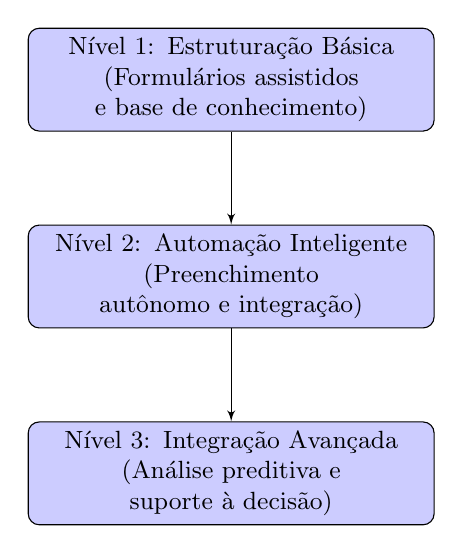
\begin{tikzpicture}[node distance=1.8cm, auto]
    % Definição dos estilos
    \tikzstyle{block} = [rectangle, draw, fill=blue!20, text width=14em, text centered, rounded corners, minimum height=3em, font=\small]
    \tikzstyle{line} = [draw, -latex']
    
    % Nós
    \node [block] (nivel1) {Nível 1: Estruturação Básica\\(Formulários assistidos e base de conhecimento)};
    \node [block, below of=nivel1, node distance=2.5cm] (nivel2) {Nível 2: Automação Inteligente\\(Preenchimento autônomo e integração)};
    \node [block, below of=nivel2, node distance=2.5cm] (nivel3) {Nível 3: Integração Avançada\\(Análise preditiva e suporte à decisão)};
    
    % Conexões
    \path [line] (nivel1) -- (nivel2);
    \path [line] (nivel2) -- (nivel3);
\end{tikzpicture}
\caption{Níveis de Implementação da Solução}
\end{figure}

\textbf{Componentes principais da solução:}

\begin{enumerate}
    \item \textbf{Interfaces de usuário:}
    \begin{itemize}
        \item Interface conversacional via WhatsApp: Canal principal de interação para maior acessibilidade
        \item Portal web responsivo: Interface alternativa com recursos visuais avançados
        \item Integração com SEI: Conexão com o sistema oficial de tramitação de processos
    \end{itemize}
    
    \item \textbf{Backend inteligente:}
    \begin{itemize}
        \item Recebimento de webhooks da API do WhatsApp: Integração utilizando Meta Cloud API ou APIs abstratas como ManyChat ou Z-API
        \item Conexão com banco de dados: Armazenamento centralizado das informações recebidas
        \item Motor de processamento de linguagem natural: Implementação baseada em AWS Bedrock
        \item Base de conhecimento vetorial: Busca semântica em documentos técnicos
        \item Sistema de formulários inteligentes: Validação em tempo real e preenchimento assistido
        \item Orquestrador de processos: Gestão integrada dos fluxos e integrações
    \end{itemize}
    
    \item \textbf{Integração com o SEI:}
    \begin{itemize}
        \item A integração com o SEI será flexível, adaptando-se às diversas implementações devido à falta de padronização nacional
        \item Abordagem híbrida:
        \begin{itemize}
            \item Uso da API oficial (quando disponível): Integração via RESTful API com autenticação segura e padronizada
            \item Exemplo: SEI-SP (\url{https://sei.prefeitura.sp.gov.br/api})
            \item Automação via Selenium (ausência de API oficial): Simulação do usuário utilizando ferramentas como Selenium ou Playwright
            \item Navegação, preenchimento de formulários, envio de documentos e acompanhamento automatizado com logs detalhados e segurança
        \end{itemize}
    \end{itemize}
    
    \item \textbf{Repositório de conhecimento:}
    \begin{itemize}
        \item Documentação técnica: Normas, procedimentos, manuais e referências
        \item Templates de formulários: Modelos padronizados para diferentes tipos de solicitação
        \item Base de casos: Histórico de solicitações anteriores para referência e aprendizado
        \item FISPQ e documentação de produtos químicos: Catálogo digital de informações de segurança
    \end{itemize}
    
    \item \textbf{Módulos analíticos:}
    \begin{itemize}
        \item Dashboard de indicadores: Para monitoramento de KPIs
        \item Sistema de alertas: Para notificação proativa de prazos e pendências
        \item Módulo de relatórios: Para geração automática de relatórios gerenciais
        \item Análise de tendências: Para identificação preventiva de riscos
    \end{itemize}
\end{enumerate}

\textbf{Requisitos funcionais prioritários:}

\begin{itemize}
    \item Capacidade de interação em linguagem natural para orientar usuários
    \item Preenchimento assistido de formulários com validação em tempo real
    \item Consulta a base de conhecimento para responder dúvidas frequentes
    \item Integração com o SEI para submissão e acompanhamento de processos
    \item Notificação automática para equipe técnica e solicitantes
    \item Geração assistida de relatórios e documentos técnicos
    \item Gestão de documentos com versionamento e controle de acesso
    \item Análise e visualização de dados de segurança do trabalho
\end{itemize}

\textbf{Requisitos não-funcionais:}

\begin{itemize}
    \item Segurança: Proteção de dados sensíveis conforme LGPD
    \item Disponibilidade: Acesso 24/7 com pelo menos 99,5\% de uptime
    \item Desempenho: Tempo de resposta inferior a 2 segundos
    \item Escalabilidade: Capacidade para atender todos os campi do IFPE
    \item Usabilidade: Interface intuitiva para usuários com diferentes níveis de familiaridade tecnológica
    \item Manutenibilidade: Facilidade de atualização e expansão
    \item Interoperabilidade: Integração com sistemas existentes
\end{itemize}

\subsection{Estratégia de Implantação}

\subsubsection{Análise SWOT}

Para definir a estratégia mais adequada de implantação, realizamos uma análise SWOT, apresentada a seguir.

\begin{table}[htbp]
\centering
\begin{tcolorbox}[enhanced, colback=green!5, colframe=green!40!black, arc=3mm, boxrule=0.5pt, width=0.85\textwidth]
\begin{tabular}{|p{12cm}|}
\hline
\rowcolor{green!10}\large \textbf{Forças (Strengths)} \\
\hline
\begin{itemize}\setlength{\itemsep}{1pt}
\item Área de segurança bem regulamentada, facilitando a criação de padrões e regras para o chatbot
\item Especialista (César) engajado e conhecedor dos processos
\item Apoio da alta administração do IFPE
\item Processos relativamente estáveis e bem definidos
\item Tecnologias de IA maduras disponíveis para implementação
\item Equipe de projeto multidisciplinar
\end{itemize} \\
\hline
\end{tabular}
\end{tcolorbox}
\caption{Análise SWOT - Forças do Projeto}
\end{table}

\begin{table}[htbp]
\centering
\begin{tcolorbox}[enhanced, colback=red!5, colframe=red!40!black, arc=3mm, boxrule=0.5pt, width=0.85\textwidth]
\begin{tabular}{|p{12cm}|}
\hline
\rowcolor{red!10}\large \textbf{Fraquezas (Weaknesses)} \\
\hline
\begin{itemize}\setlength{\itemsep}{1pt}
\item Equipe técnica reduzida no setor de segurança de trabalho
\item Resistência à mudança de processos estabelecidos
\item Dependência de Infraestrutura de TI
\item Lacunas na documentação atual dos processos
\item Complexidade de integração com sistemas legados (SEI)
\item Recursos financeiros limitados da instituição pública
\end{itemize} \\
\hline
\end{tabular}
\end{tcolorbox}
\caption{Análise SWOT - Fraquezas do Projeto}
\end{table}

\begin{table}[htbp]
\centering
\begin{tcolorbox}[enhanced, colback=blue!5, colframe=blue!40!black, arc=3mm, boxrule=0.5pt, width=0.85\textwidth]
\begin{tabular}{|p{12cm}|}
\hline
\rowcolor{blue!10}\large \textbf{Oportunidades (Opportunities)} \\
\hline
\begin{itemize}\setlength{\itemsep}{1pt}
\item Crescente aceitação de interfaces conversacionais (chatbot)
\item Possibilidade de expansão futura para outros domínios (saúde)
\item Projeto piloto pode servir de modelo para outras instituições
\item Evolução rápida das tecnologias de IA
\item Melhoria da imagem institucional por inovação tecnológica
\end{itemize} \\
\hline
\end{tabular}
\end{tcolorbox}
\caption{Análise SWOT - Oportunidades do Projeto}
\end{table}

\begin{table}[htbp]
\centering
\begin{tcolorbox}[enhanced, colback=yellow!5, colframe=yellow!40!black, arc=3mm, boxrule=0.5pt, width=0.85\textwidth]
\begin{tabular}{|p{12cm}|}
\hline
\rowcolor{yellow!10}\large \textbf{Ameaças (Threats)} \\
\hline
\begin{itemize}\setlength{\itemsep}{1pt}
\item Restrições orçamentárias imprevistas
\item Problemas de segurança de dados e conformidade com a LGPD
\item Resistência cultural à adoção de IA no setor público
\item Greve ou paralisações que afetem o cronograma
\item Mudança na gestão do IFPE que afetem as prioridades
\end{itemize} \\
\hline
\end{tabular}
\end{tcolorbox}
\caption{Análise SWOT - Ameaças do Projeto}
\end{table}
\subsubsection{Estratégia selecionada}

Com base na análise SWOT e nas características do projeto, selecionamos uma estratégia de implantação \textbf{gradual e iterativa}, com as seguintes características:

\begin{enumerate}
    \item \textbf{Abordagem gradual em níveis:} Implementação em três níveis progressivos (Estruturação Básica, Automação Inteligente, Integração Avançada), conforme definido anteriormente.
    
    \item \textbf{Implantação por processos prioritários:} Início pelos processos mais críticos e de maior impacto, conforme identificado na matriz de processos suportados.
    
    \item \textbf{Programa piloto:} Seleção de um grupo inicial de usuários para validação antes da expansão para toda a instituição.
    
    \item \textbf{Ciclos de feedback contínuo:} Coleta e incorporação de feedback dos usuários ao longo de todo o processo.
    
    \item \textbf{Desenvolvimento ágil:} Utilização de metodologias ágeis para permitir ajustes e adaptações durante a implementação.
\end{enumerate}

\textbf{Justificativa da estratégia:}

Esta estratégia foi selecionada com base nos seguintes fatores identificados na análise SWOT:

\begin{itemize}
    \item \textbf{Mitigação de riscos:} A abordagem gradual permite identificar e corrigir problemas em estágios iniciais, sem comprometer todo o projeto.
    
    \item \textbf{Adaptação à cultura organizacional:} A implementação progressiva respeita o ritmo de adaptação da instituição, reduzindo a resistência à mudança.
    
    \item \textbf{Otimização de recursos limitados:} A priorização de processos críticos garante que os recursos sejam alocados para as áreas de maior impacto.
    
    \item \textbf{Aprendizado contínuo:} Os ciclos de feedback permitem o refinamento da solução com base na experiência real dos usuários.
    
    \item \textbf{Flexibilidade diante de incertezas:} A abordagem ágil proporciona flexibilidade para lidar com mudanças de contexto ou prioridades.
\end{itemize}

\subsubsection{Infraestrutura necessária}

A implementação do chatbot com IA para processos de segurança do trabalho requer a seguinte infraestrutura:

\begin{table}[H]
\centering
\begin{adjustbox}{max width=\textwidth}
\renewcommand{\arraystretch}{1.2}
\begin{tabular}{|p{3cm}|p{5cm}|p{4cm}|p{3cm}|}
\hline
\rowcolor{gray!20}
\textbf{Categoria} & \textbf{Recursos} & \textbf{Especificações} & \textbf{Fase Necessária} \\
\hline
\multirow{3}{*}{Servidores} & Ambiente de Desenvolvimento & Servidor virtual com 8 vCPUs, 16GB RAM, 100GB SSD & Preparação \\
\cline{2-4}
 & Ambiente de Homologação & Servidor virtual com 8 vCPUs, 16GB RAM, 100GB SSD & Piloto \\
\cline{2-4}
 & Ambiente de Produção & Servidor virtual com 16 vCPUs, 32GB RAM, 500GB SSD & Expansão \\
\hline
\multirow{3}{*}{Serviços em Nuvem} & AWS Bedrock & API para modelos de IA como Claude Opus & Todas \\
\cline{2-4}
 & Amazon S3 & Armazenamento de documentos e artefatos & Todas \\
\cline{2-4}
 & Amazon RDS & Banco de dados relacional & Todas \\
\hline
\multirow{2}{*}{Canais de Comunicação} & API WhatsApp Business & Licença para envio de mensagens em volume & Piloto em diante \\
\cline{2-4}
 & Domínio e SSL & Certificados para portal web & Preparação \\
\hline
\multirow{2}{*}{Segurança} & Soluções de Backup & Backup diário com retenção de 30 dias & Todas \\
\cline{2-4}
 & Ferramentas de Monitoramento & Sistema de logs e alertas & Todas \\
\hline
\multirow{2}{*}{Desenvolvimento} & Ambientes de Desenvolvimento & Acesso aos ambientes e ferramentas de desenvolvimento & Preparação \\
\cline{2-4}
 & Repositório de Código & Sistema de controle de versão (Git) & Preparação \\
\hline
\end{tabular}
\end{adjustbox}
\caption{Infraestrutura Necessária para Implantação}
\end{table}

\subsubsection{Metodologia de trabalho}

Para garantir uma implementação bem-sucedida, adotaremos a seguinte metodologia de trabalho:

\begin{enumerate}
    \item \textbf{Gestão de projeto:} Utilização do framework Scrum adaptado, com sprints de duas semanas e reuniões diárias de sincronização.
    
    \item \textbf{Monitoramento de progresso:} Utilização de quadro Kanban para visualização do fluxo de trabalho e acompanhamento de tarefas.
    
    \item \textbf{Reuniões regulares:}
    \begin{itemize}
        \item Reuniões diárias (15 minutos): Sincronização da equipe de desenvolvimento
        \item Reuniões semanais (1 hora): Acompanhamento com stakeholders principais
        \item Reuniões quinzenais (2 horas): Demonstração de incrementos e coleta de feedback
        \item Reuniões mensais (3 horas): Revisão de progresso e planejamento estratégico
    \end{itemize}
    
    \item \textbf{Documentação:}
    \begin{itemize}
        \item Backlog do produto: Lista priorizada de requisitos e funcionalidades
        \item Documentação técnica: Arquitetura, integrações e configurações
        \item Atas de reunião: Registro das decisões e próximos passos
        \item Relatórios de progresso: Status do projeto, riscos e planos de mitigação
    \end{itemize}
    
    \item \textbf{Comunicação:}
    \begin{itemize}
        \item E-mail corporativo: Para comunicações formais e documentação
        \item Grupo de mensagens instantâneas: Para comunicação rápida e alinhamentos
        \item Reuniões virtuais: Para discussões e demonstrações
        \item Portal do projeto: Para compartilhamento de artefatos e acompanhamento
    \end{itemize}
    
    \item \textbf{Validação e testes:}
    \begin{itemize}
        \item Testes unitários: Validação de componentes individuais
        \item Testes de integração: Verificação da interação entre componentes
        \item Testes de usuário: Validação da experiência do usuário com cenários reais
        \item Homologação: Aprovação formal pelos stakeholders
    \end{itemize}
\end{enumerate}

\clearpage
\subsection{Dimensionamento e Perfil da Equipe para a Implantação da Melhoria}

A implantação do chatbot com IA para processos de segurança do trabalho requer uma equipe multidisciplinar com diferentes competências. A seguir, detalhamos o dimensionamento e o perfil necessários:

\begin{table}[htbp]
\centering
\renewcommand{\arraystretch}{1.2}
\resizebox{0.95\textwidth}{!}{
\begin{tabular}{|p{3cm}|p{3cm}|p{3cm}|p{6cm}|}
\hline
\rowcolor{gray!20}
\textbf{Papel} & \textbf{Quantidade} & \textbf{Dedicação} & \textbf{Responsabilidades} \\
\hline
Gerente de Projeto & 1 & 100\% & Coordenação geral, gestão de recursos, comunicação com stakeholders, gerenciamento de riscos \\
\hline
Arquiteto de Soluções & 1 & 50\% & Definição da arquitetura técnica, seleção de tecnologias, planejamento de integrações \\
\hline
Especialista em IA & 1 & 50\% & Treinamento de modelos, configuração de APIs de IA, otimização de desempenho \\
\hline
Desenvolvedor Full Stack & 2 & 100\% & Desenvolvimento de front-end, back-end e integrações \\
\hline
Engenheiro de Dados & 1 & 50\% & Modelagem de dados, ETL, estruturação da base de conhecimento \\
\hline
Designer UX/UI & 1 & 50\% & Design de interfaces, jornadas de usuário, testes de usabilidade \\
\hline
Especialista em Segurança & 1 & 30\% & Implementação de controles de segurança, conformidade com LGPD \\
\hline
Analista de Qualidade & 1 & 50\% & Testes, validação de requisitos, garantia de qualidade \\
\hline
Especialista em Segurança do Trabalho & 1 & 30\% & Validação técnica, fornecimento de conteúdo, homologação funcional \\
\hline
Analista de Negócios & 1 & 50\% & Levantamento de requisitos, modelagem de processos, interface com usuários \\
\hline
\end{tabular}
}
\caption{Dimensionamento e Perfil da Equipe}
\end{table}
\clearpage

\subsection{Custos Associados à Implantação da Melhoria}

A estimativa de custos para a implantação do chatbot com IA para processos de segurança do trabalho foi calculada considerando os recursos humanos, infraestrutura, licenças e serviços necessários:

\begin{table}[htbp]
\centering
\resizebox{0.9\textwidth}{!}{
\begin{tabular}{|p{2.8cm}|p{3.2cm}|r|r|}
\hline
\rowcolor{gray!20}
\textbf{Categoria} & \textbf{Item} & \textbf{Valor Mensal (R\$)} & \textbf{Valor Total (R\$)} \\
\hline
\multirow{3}{*}{Recursos Humanos} & Equipe interna (dedicação parcial) & 0,00 & 0,00 \\
\cline{2-4}
 & Suporte técnico (3 meses) & 2.000,00 & 6.000,00 \\
\cline{2-4}
 & \textbf{Subtotal RH} & & \textbf{6.000,00} \\
\hline
\multirow{3}{*}{Infraestrutura e Serviços} & Servidor virtual compartilhado & 300,00 & 900,00 \\
\cline{2-4}
 & API de IA (Claude/OpenAI) & 500,00 & 1.500,00 \\
\cline{2-4}
 & \textbf{Subtotal Infraestrutura} & & \textbf{2.400,00} \\
\hline
\multirow{3}{*}{Licenças e Ferramentas} & API WhatsApp Business & 1.000,00 & 3.000,00 \\
\cline{2-4}
 & Bibliotecas open-source & 0,00 & 0,00 \\
\cline{2-4}
 & \textbf{Subtotal Licenças} & & \textbf{3.000,00} \\
\hline
\multirow{4}{*}{Outros Custos} & Treinamento de usuários & - & 3.000,00 \\
\cline{2-4}
 & Documentação e materiais & - & 3.800,00 \\
\cline{2-4}
 & Contingência (10\%) & - & 1.800,00 \\
\cline{2-4}
 & \textbf{Subtotal Outros} & & \textbf{8.600,00} \\
\hline
\multicolumn{2}{|r|}{\textbf{TOTAL}} & & \textbf{20.000,00} \\
\hline
\end{tabular}
}
\caption{Custos Associados à Implantação}
\end{table}

\textbf{Observações sobre os custos:}
\begin{itemize}
    \item A estimativa foi otimizada para um orçamento reduzido de R\$ 20.000,00
    \item A implementação será realizada utilizando principalmente recursos internos do IFPE, sem custo adicional
    \item Adotaremos abordagem baseada em software livre e APIs de baixo custo
    \item Utilizaremos infraestrutura já existente na instituição, minimizando novos investimentos em hardware
    \item O desenvolvimento será conduzido por equipe interna com suporte técnico limitado
    \item As integrações com sistemas existentes serão feitas de forma progressiva, reduzindo custos iniciais
    \item O projeto será implementado seguindo metodologia ágil, priorizando funcionalidades de maior valor
\end{itemize}

\subsection{Cronograma Macro}

O cronograma macro para a implantação do chatbot com IA para processos de segurança do trabalho está organizado em quatro fases principais, com duração total de 22 semanas:

\begin{landscape}
\begin{table}[htbp]
\centering
\renewcommand{\arraystretch}{1.1}
\begin{tabular}{|p{2cm}|p{1.2cm}|p{7cm}|p{6cm}|}
\hline
\rowcolor{gray!20}
\textbf{Fase} & \textbf{Duração} & \textbf{Principais Atividades} & \textbf{Entregas} \\
\hline
\multirow{4}{*}{Preparação} & \multirow{4}{*}{4 sem.} & $\bullet$ Definição de requisitos & $\bullet$ Requisitos aprovados \\
\cline{3-4}
 & & $\bullet$ Configuração da infraestrutura & $\bullet$ Ambientes configurados \\
\cline{3-4}
 & & $\bullet$ Treinamento inicial da IA & $\bullet$ Base de conhecimento inicial \\
\cline{3-4}
 & & $\bullet$ Definição de métricas & $\bullet$ Framework de avaliação \\
\hline
\multirow{4}{*}{Piloto} & \multirow{4}{*}{6 sem.} & $\bullet$ Desenvolvimento do Nível 1 & $\bullet$ Chatbot básico \\
\cline{3-4}
 & & $\bullet$ Seleção e treinamento de usuários piloto & $\bullet$ Grupo piloto treinado \\
\cline{3-4}
 & & $\bullet$ Teste com grupo piloto & $\bullet$ Relatório de feedback \\
\cline{3-4}
 & & $\bullet$ Ajustes baseados no feedback & $\bullet$ Versão refinada do Nível 1 \\
\hline
\multirow{4}{*}{Expansão} & \multirow{4}{*}{8 sem.} & $\bullet$ Desenvolvimento do Nível 2 & $\bullet$ Funcionalidades de automação \\
\cline{3-4}
 & & $\bullet$ Treinamento de multiplicadores & $\bullet$ Equipe de multiplicadores formada \\
\cline{3-4}
 & & $\bullet$ Implantação em departamentos selecionados & $\bullet$ Solução disponível para áreas selecionadas \\
\cline{3-4}
 & & $\bullet$ Integração com sistemas existentes & $\bullet$ Conectores funcionais com SEI \\
\hline
\multirow{4}{*}{Consolidação} & \multirow{4}{*}{4 sem.} & $\bullet$ Desenvolvimento de recursos do Nível 3 & $\bullet$ Funcionalidades avançadas \\
\cline{3-4}
 & & $\bullet$ Implantação geral & $\bullet$ Solução disponível para toda instituição \\
\cline{3-4}
 & & $\bullet$ Avaliação de resultados & $\bullet$ Relatório de desempenho \\
\cline{3-4}
 & & $\bullet$ Planejamento de melhorias contínuas & $\bullet$ Roadmap de evolução \\
\hline
\end{tabular}
\caption{Cronograma Macro de Implantação}
\end{table}
\end{landscape}

\begin{table}[htbp]
\centering
\resizebox{\textwidth}{!}{
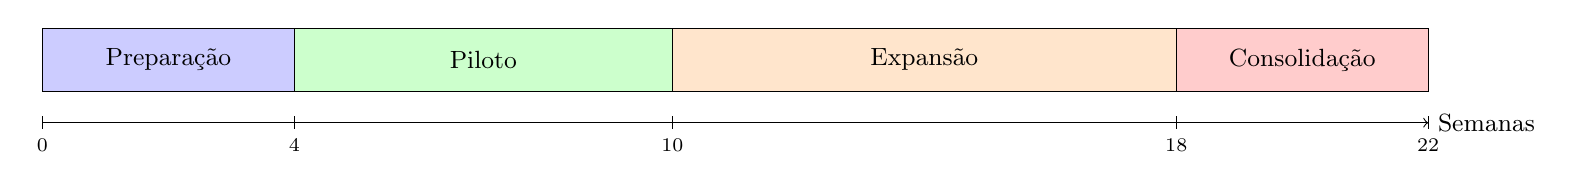
\begin{tikzpicture}[scale=0.8]
\draw[->] (0,0) -- (22,0) node[right] {\small Semanas};
\foreach \x in {0,4,10,18,22}
    \draw (\x,0.1) -- (\x,-0.1) node[below] {\scriptsize \x};

\filldraw[fill=blue!20] (0,0.5) rectangle (4,1.5) node[midway, font=\small] {Preparação};
\filldraw[fill=green!20] (4,0.5) rectangle (10,1.5) node[midway, font=\small] {Piloto};
\filldraw[fill=orange!20] (10,0.5) rectangle (18,1.5) node[midway, font=\small] {Expansão};
\filldraw[fill=red!20] (18,0.5) rectangle (22,1.5) node[midway, font=\small] {Consolidação};
\end{tikzpicture}
}
\caption{Linha do Tempo do Projeto}
\end{table}

\clearpage
\subsection{Plano de medições e análise}

Para avaliar o sucesso da implantação e os benefícios entregues pela solução, estabelecemos um conjunto de indicadores-chave de desempenho (KPIs) que serão monitorados ao longo do projeto:

\subsubsection{Indicador: Tempo médio de preenchimento de formulários}

\textbf{Finalidade:} Avaliar a eficiência da solução na redução do tempo necessário para preencher formulários relacionados à segurança do trabalho.

\textbf{Como medir:} 
\begin{itemize}
    \item Linha base: Medição do tempo médio atual através de observação direta e entrevistas (estimado em 45 minutos)
    \item Pós-implantação: Registro automático do tempo entre início e conclusão do preenchimento via chatbot
    \item Frequência: Mensal
\end{itemize}

\textbf{Análise de impacto:} A redução do tempo de preenchimento tem impacto direto na produtividade dos servidores e na agilidade dos processos. A meta é reduzir em 67\% (para 15 minutos) em 12 meses.

\subsubsection{Indicador: Taxa de preenchimento correto na primeira tentativa}

\textbf{Finalidade:} Avaliar a eficácia da solução na redução de erros e retrabalho.

\textbf{Como medir:} 
\begin{itemize}
    \item Linha base: Percentual de formulários que precisam ser corrigidos ou complementados (estimado em 40\% de acerto)
    \item Pós-implantação: Registro automático de formulários completos e válidos na primeira submissão
    \item Frequência: Mensal
\end{itemize}

\textbf{Análise de impacto:} O aumento da taxa de acerto reduz retrabalho tanto para solicitantes quanto para a equipe técnica. A meta é aumentar para 80\% em 12 meses.

\subsubsection{Indicador: Consultas básicas direcionadas à equipe técnica}

\textbf{Finalidade:} Avaliar o grau de desoneração da equipe técnica de atividades de baixo valor agregado.

\textbf{Como medir:} 
\begin{itemize}
    \item Linha base: Contagem de consultas básicas semanais recebidas pela equipe técnica (estimado em 35)
    \item Pós-implantação: Registro de consultas não resolvidas pelo chatbot
    \item Frequência: Semanal
\end{itemize}

\textbf{Análise de impacto:} A redução de consultas básicas permite que a equipe técnica se concentre em atividades que exigem expertise especializada. A meta é reduzir para 8 consultas semanais em 12 meses.

\subsubsection{Indicador: Dúvidas atendidas sem intervenção humana}

\textbf{Finalidade:} Avaliar a autonomia e eficácia do chatbot.

\textbf{Como medir:} 
\begin{itemize}
    \item Linha base: Percentual de dúvidas que podem ser resolvidas automaticamente (estimado em 20\%)
    \item Pós-implantação: Percentual de consultas resolvidas pelo chatbot sem escalação
    \item Frequência: Mensal
\end{itemize}

\textbf{Análise de impacto:} O aumento da resolução automática amplia a disponibilidade do serviço e reduz dependência de recursos humanos limitados. A meta é aumentar para 80\% em 12 meses.

\subsubsection{Indicador: Satisfação do usuário}

\textbf{Finalidade:} Avaliar a percepção dos usuários sobre a qualidade e utilidade da solução.

\textbf{Como medir:} 
\begin{itemize}
    \item Linha base: Pesquisa de satisfação com serviços atuais (estimado em 65\%)
    \item Pós-implantação: Pesquisa de satisfação e feedback pós-interação com chatbot
    \item Frequência: Trimestral
\end{itemize}

\textbf{Análise de impacto:} A satisfação do usuário está diretamente relacionada à adoção e ao sucesso da solução. A meta é aumentar para 90\% em 12 meses.

\subsubsection{Indicador: Tempo de resposta para solicitações}

\textbf{Finalidade:} Avaliar a agilidade no atendimento às solicitações.

\textbf{Como medir:} 
\begin{itemize}
    \item Linha base: Tempo médio entre solicitação e resposta final (estimado em 48 horas)
    \item Pós-implantação: Registro automático do ciclo completo de solicitação
    \item Frequência: Mensal
\end{itemize}

\textbf{Análise de impacto:} A redução do tempo de resposta melhora a experiência do usuário e a eficiência operacional. A meta é reduzir para 12 horas em 12 meses.

\subsubsection{Indicador: Volume de documentação digital vs. papel}

\textbf{Finalidade:} Avaliar o grau de digitalização dos processos.

\textbf{Como medir:} 
\begin{itemize}
    \item Linha base: Percentual de documentos em formato digital (estimado em 40\%)
    \item Pós-implantação: Proporção entre documentos digitais e físicos
    \item Frequência: Trimestral
\end{itemize}

\textbf{Análise de impacto:} O aumento da digitalização facilita o acesso, reduz custos e melhora a gestão documental. A meta é aumentar para 95\% em 12 meses.

\clearpage
\section{Indicadores GPN}

Esta seção contém os indicadores de Gestão de Processos de Negócio (GPN) elaborados para o monitoramento efetivo do projeto. Conforme designado, o responsável pela criação e manutenção destes indicadores é Eric Bezerra Londres Barreto.

\begin{table}[htbp]
\centering
\resizebox{\textwidth}{!}{
\begin{tabular}{|p{3cm}|p{3cm}|p{4cm}|p{3cm}|p{3cm}|}
\hline
\rowcolor{gray!15}\textbf{Indicador} & \textbf{Métrica} & \textbf{Forma de medição} & \textbf{Valor atual} & \textbf{Meta} \\
\hline
Tempo de processamento de solicitações & Tempo médio (em dias) & Comparação entre data de abertura e conclusão & 14 dias & 3 dias \\
\hline
Taxa de conformidade documental & Percentual de documentos em conformidade & Auditoria amostral & 65\% & 95\% \\
\hline
Satisfação do usuário & Nota média (1-10) & Pesquisa pós-atendimento & 6.8 & 9.0 \\
\hline
Custo por solicitação processada & Valor em R\$ & Rateio de custos operacionais totais & R\$175,00 & R\$85,00 \\
\hline
Taxa de resolução automatizada & Percentual de solicitações resolvidas sem intervenção humana & Relatórios do sistema & 0\% & 70\% \\
\hline
Tempo de resposta a emergências & Tempo médio (em horas) & Log do sistema para casos prioritários & 12h & 2h \\
\hline
\end{tabular}
}
\caption{Indicadores GPN do Projeto}
\end{table}

Estes indicadores serão monitorados regularmente ao longo da implementação e operação do sistema, com relatórios mensais apresentados à equipe de gerenciamento do projeto e relatórios trimestrais aos stakeholders. A planilha completa com o acompanhamento histórico e detalhado destes indicadores é mantida por Eric Barreto e está disponível no repositório do projeto.

\clearpage
\section{Conclusões e Considerações Finais}

A implantação do chatbot com IA para processos de segurança do trabalho representa uma oportunidade significativa para transformar e modernizar os serviços prestados pelo setor de Segurança do Trabalho do SIASS/IFPE. Este plano de implantação foi elaborado com base em uma análise detalhada do contexto atual, identificação de desafios e oportunidades, e definição de uma estratégia gradual e iterativa para maximizar as chances de sucesso.

Os principais benefícios esperados com a implementação desta solução incluem:

\begin{itemize}
    \item \textbf{Eficiência operacional:} Redução significativa no tempo de processamento de solicitações e no esforço administrativo da equipe técnica.
    
    \item \textbf{Padronização e qualidade:} Maior consistência nos processos e documentos, com redução de erros e retrabalho.
    
    \item \textbf{Acessibilidade:} Disponibilização de informações e serviços de forma mais acessível e intuitiva para todos os servidores.
    
    \item \textbf{Preservação do conhecimento:} Estruturação e centralização do conhecimento técnico em segurança do trabalho.
    
    \item \textbf{Inteligência organizacional:} Geração de dados e insights para tomada de decisão baseada em evidências.
    
    \item \textbf{Evolução tecnológica:} Posicionamento do IFPE como instituição inovadora na aplicação de tecnologias avançadas para melhoria de serviços.
\end{itemize}

Para garantir o sucesso desta iniciativa, algumas considerações importantes devem ser observadas:

\begin{enumerate}
    \item \textbf{Gestão da mudança:} É fundamental investir em comunicação, treinamento e envolvimento dos usuários desde as fases iniciais do projeto.
    
    \item \textbf{Flexibilidade:} O plano deve ser adaptável para acomodar aprendizados e necessidades emergentes ao longo da implementação.
    
    \item \textbf{Foco no valor:} As decisões devem sempre priorizar o valor entregue aos usuários e à instituição, não apenas aspectos técnicos.
    
    \item \textbf{Visão de longo prazo:} Embora implementado em fases, o projeto deve manter alinhamento com a visão estratégica de longo prazo.
    
    \item \textbf{Sustentabilidade:} A solução deve ser projetada para ser mantida e evoluída após a conclusão do projeto inicial.
\end{enumerate}

A estratégia de implementação em três níveis progressivos permite uma abordagem controlada e sustentável, minimizando riscos e maximizando o aprendizado. Iniciando com funcionalidades básicas de preenchimento assistido de formulários e base de conhecimento, evoluindo para automação inteligente e integração de sistemas, e finalmente alcançando recursos avançados de análise preditiva e suporte à decisão, o projeto oferece entregas de valor em cada etapa.

O sucesso desta iniciativa não depende apenas de aspectos tecnológicos, mas principalmente do engajamento das pessoas e da capacidade de integrar a solução aos processos e à cultura da instituição. O comprometimento da alta administração, a participação ativa dos especialistas em segurança do trabalho e a adoção pelos usuários finais são fatores críticos para que os benefícios esperados sejam plenamente alcançados.

Recomenda-se o início imediato da fase de preparação, seguindo o cronograma e a metodologia definidos neste plano, com acompanhamento regular dos indicadores estabelecidos para avaliar o progresso e o impacto da solução.

\clearpage
\section*{Assinaturas}

Concordamos com o plano de implantação apresentado neste documento:

\vspace{1cm}

\begin{table}[htbp]
\centering
\begin{tabular}{p{7cm}p{7cm}}
\makebox[7cm]{\hrulefill} & \makebox[7cm]{\hrulefill} \\
Pedro Henrique Souza Balbino & Eric Bezerra Londres Barreto \\
Analista de Processos / Gerente de Projeto & Arquiteto de Soluções / Especialista em IA \\[2em]

\makebox[7cm]{\hrulefill} & \makebox[7cm]{\hrulefill} \\
Lucas Lucena Xavier de Morais & Sara Simone Emilay de Araujo Pereira \\
Desenvolvedor / Integração de Sistemas / Gestor desse último ciclo & Analista de Requisitos / Gestão da Mudança \\[2em]

\makebox[7cm]{\hrulefill} & \makebox[7cm]{\hrulefill} \\
Luis Felipe Guedes Souto Moreira & Maria Beatriz Martins Pontes Gonçalo \\
Desenvolvedor / Engenheiro de Dados & Designer de UX/UI / Gestora desse último ciclo \\[2em]

\makebox[7cm]{\hrulefill} & \makebox[7cm]{\hrulefill} \\
Pablo Henrique Ferreira da Silva & Vinicius Nobre da Silva Prazeres \\
Especialista em Segurança da Informação & Analista de Qualidade / Testes \\[2em]

\makebox[7cm]{\hrulefill} & \\
César de Oliveira & \\
Especialista em Segurança do Trabalho - SIASS/IFPE & \\
\end{tabular}
\end{table}

\end{document}